\section{Results}
\label{sec:results}

\paragraph{Validity.}
All \TurnsPerModel{} turns completed on each model and no turn was excluded.
The two recompute arms were bit-identical on every turn (\FloorInexact{} of
\TurnsTotal{} differed), so the engine was deterministic and any difference is
attributable to restore. Every restore result reproduced in its second
replicate, and no action change appeared in only one replicate.

\paragraph{Exactness.}
At natural boundaries, \NatInexact{} of \NatTurns{} restores were not
bit-exact (a descriptive count). That includes all \ExplicitTurns{} explicit-request turns, where
restore and recompute generated identical tokens but never identical
log-probabilities. At snapped boundaries (confirmatory, H1) every restore was bit-exact on Ornith
and on Qwen3 (\SnapValidOrnith{} of \SnapValidOrnith{} turns each). On Spark,
the 180 short-history turns were exact and all \SnapInexactSpark{} long-history
turns were not, which falsifies H1 for that model.

\begin{figure}[t]
\centering
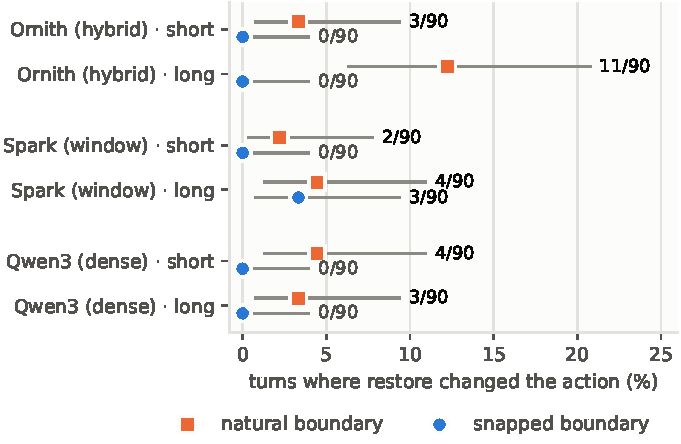
\includegraphics[width=\columnwidth]{figures/action_changes.pdf}
\caption{Turns on which restore changed the agent's action, on ambiguous
requests (confirmatory, family~A). Each point is 90 turns; bars are 95\%
Clopper--Pearson intervals. Ornith is the hybrid recurrent model, Spark the
sliding-window model, Qwen3 the dense model. On explicit requests there were
\ExplicitChanges{} changes in \ExplicitRestores{} restores.}
\label{fig:actions}
\end{figure}

\paragraph{Action changes (confirmatory).}
Figure~\ref{fig:actions} shows family~A. At natural boundaries, restore changed
the action on ambiguous requests on every model:
on Ornith, \AOrnithNatShortAmb{} of \AOrnithNatShortAmbN{} short-history turns
(\AOrnithNatShortAmbPct\%, 95\% CI \AOrnithNatShortAmbLo--\AOrnithNatShortAmbHi\%)
and \AOrnithNatLongAmb{} of \AOrnithNatLongAmbN{} long-history turns
(\AOrnithNatLongAmbPct\%, CI \AOrnithNatLongAmbLo--\AOrnithNatLongAmbHi\%);
on Spark, \ASparkNatShortAmb{} (\ASparkNatShortAmbPct\%) and
\ASparkNatLongAmb{} (\ASparkNatLongAmbPct\%);
on Qwen3, \AQwenNatShortAmb{} (\AQwenNatShortAmbPct\%) and
\AQwenNatLongAmb{} (\AQwenNatLongAmbPct\%).
No explicit request changed: \ExplicitChanges{} of \ExplicitRestores{} restores,
with a 95\% upper bound of \AOrnithNatShortExpHi\% per cell of 90. At snapped
boundaries the only changes were \ASparkSnapLongAmb{} on Spark's long
histories. In total \ClaimedA{} of the \MembersA{} family members are claimed.
The dense and sliding-window models changed actions too, at rates similar to
the hybrid's on short histories. The study pre-registered no test that compares
action-change rates between architectures, and with 2--11 events per cell the
intervals overlap widely.

\begin{figure}[t]
\centering
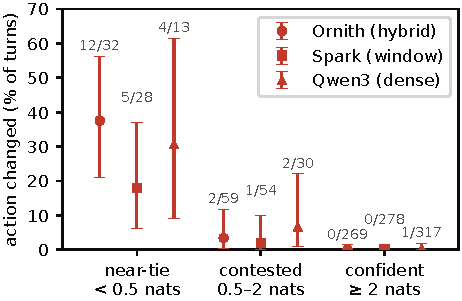
\includegraphics[width=\columnwidth]{figures/margin_bins.pdf}
\caption{Action changes at natural boundaries by the recompute arm's action
margin (pre-registered secondary; intervals only). Labels give changed turns
over turns in the bin; bars are 95\% Clopper--Pearson intervals.}
\label{fig:margins}
\end{figure}

\paragraph{Where the changes happen (pre-registered secondary).}
Figure~\ref{fig:margins} groups natural-boundary turns by action margin. Pooled
over models, restore changed the action on \MarginAllNearTie{} of
\MarginAllNearTieN{} near-tie turns (\MarginAllNearTiePct\%), \MarginAllContested{}
of \MarginAllContestedN{} contested turns (\MarginAllContestedPct\%) and
\MarginAllConfident{} of \MarginAllConfidentN{} confident turns
(\MarginAllConfidentPct\%). The predicted ordering holds on each model. This
analysis was pre-registered with intervals only, so it is descriptive.

\paragraph{What changed (descriptive).}
% src: docs/findings/2026-09-11-main-study.md, "Where the changes happen"; recounted from docs/findings/study/changed_turns.json
Of the \ChangesTotal{} changes, 11 were the same tool called with different
arguments, 10 were a tool call that became a text reply, and 9 were a text
reply or clarifying question that became a tool call. None switched to a
different tool. In one case both arms summed a list of 23 numbers from the
history, but the restore arm omitted one of them, so the tool returned a
different total (Appendix~\ref{app:examples}).

\paragraph{Distribution drift (confirmatory).}
Restore shifted the hybrid's output distribution at every natural boundary
(family~B, all eight natural-boundary members claimed; H2). On explicit
requests with short histories the median per-turn mean JSD (descriptive) was
$\DriftOrnithShortExp$ on Ornith against $\DriftQwenShortExp$ on Qwen3 and
$\DriftSparkShortExp$ on Spark. Of the six contrasts in family~C, three are
claimed: snapping removes drift on the hybrid (C1), the hybrid drifts more than
the sliding-window model (C4), and action changes are more frequent on
ambiguous than explicit requests (C6). The hybrid drifted more than the dense
model on \CThreePos{} of 360 turns, but the interval of the mean difference
includes zero ($[\CThreeLo, \CThreeHi]$), so C3 is not claimed: a few
dense-model turns drifted heavily. Drift was not shown
to grow with history length (C5). The models see different prompt lengths for
the same conversation (Table~\ref{tab:setup}); in an exploratory check within
each history length, the hybrid still drifted more than the sliding-window
model.
Appendix~\ref{app:families} has the full tables.

\begin{table}[t]
\caption{Pre-registered hypotheses and verdicts. A hypothesis is supported only
if every test it names is claimed.}
\label{tab:hypotheses}
% src: docs/findings/2026-09-11-main-study.md, "Hypotheses"
\small
\begin{tabular}{@{}l>{\raggedright\arraybackslash}p{0.46\columnwidth}>{\raggedright\arraybackslash}p{0.36\columnwidth}@{}}
\toprule
 & Hypothesis & Verdict \\
\midrule
H1 & Snapped restores are bit-exact on every model & Holds on hybrid and dense; \textbf{fails} on sliding window \\
H2 & Restore shifts the hybrid's output distribution & Supported \\
H3 & Restore changes the hybrid's actions & Partial: ambiguous requests only \\
H4 & The hybrid diverges more than both controls & Partial: more than sliding window; not shown for dense \\
H5 & Snapping helps, more on the hybrid than the dense model & Partial: helps; a larger effect on the hybrid not shown \\
H6 & Divergence grows with history length & \textbf{Not supported} \\
H7 & Action changes concentrate in ambiguous requests & Supported \\
\bottomrule
\end{tabular}
\end{table}
